\documentclass[a4paper,sffamily,12pt]{article}

\usepackage[T1]{fontenc}
\usepackage[french]{babel}
\usepackage[utf8]{inputenc}

% Customization des listes
\usepackage{enumitem}
\usepackage{pifont}

% Insertion d'image
\usepackage{graphicx}

% Création de lien
\usepackage[colorlinks,linkcolor=blue]{hyperref}

% Formatage des titres de sections
\usepackage{titlesec}
\titleformat{\section}
  {\normalfont\Large\bfseries\sffamily}{\thesection.}{0.33em}{}[\hrule]
 
 % tableau rectangle 
%\usepackage{slashbox}
%\usepackage{tabularx}

 % En-tête
\usepackage{fancyhdr}
\pagestyle{fancy}
\renewcommand\headrulewidth{1pt}
\fancyhead[L]{Base de données 2}
\fancyhead[R]{$X6I0050$}

% Permet de mettre du texte au dessus du titre
\usepackage{titling}
\renewcommand{\maketitlehooka}{\noindent MAHIER Loïc \hfill groupe 601B \\ JEHANNO Clément \hfill \\ JAMET Félix \hfill \\ PHALAVANDISHVILI  Demetre}

% Titre
\title{\vspace{\fill}\LARGE\bfseries\sffamily Rapport préliminaire de projet\protect\footnote{rapport réalisé sous \LaTeX} \vspace{\fill}}

\begin{document}

	\date{} % Supprime la date
	\maketitle % Affiche le titre

	\thispagestyle{fancy} % Permet de mettre le titre sur la page ''fancy''
	
	\newpage
			
	\renewcommand{\contentsname}{Sommaire}
	\tableofcontents
	
	\newpage
	
	\section{Introduction}
		
		\vspace{0.5cm}
		
		Dans le cadre de ce projet nous devons créer une base de données. Nous avons décidés de modéliser la gestion de cinémas sur une grande échelle. Par exemple nous voulons savoir quels sont les cinémas de France, à qui ils appartiennent (Pathé,UGC, etc.) et ce qu'ils proposent. Comme notre modèle se base sur une certaine réalité voici comment nous avons décomposé la chose, prenons  l'exemple d'un cinéma : \\
		\indent Le cinéma Pathé à Atlantis, dans la ville de Nantes. Tout d'abord on voit que un cinéma est identifié par une adresse et une ville. Ensuite, notre cinéma possède des salles dans lesquelles seront diffusés des films. Chaque film est composé d'une équipe d'acteurs, d'un réalisateur et d'une date de sortie. Il peut être compatible, ou non, à la 3D. \\ 				\indent Nos salle quant à elles, possèdent un certain nombre de places qui sont réparties entre les places "normales" et les places pour les handicapés ainsi que les nouveaux sièges dBox (sièges bougeant en même temps que le film). Si elles sont compatibles, elles ont la possibilité de diffuser en 3D. \\
		\indent Lorsqu'un film est diffusé dans une salle on appelle ça une Séance, notre séance définit le tout c'est à dire "Tel film dans tel cinéma à telle heure". Aujourd'hui si on va au cinéma il est possible de réserver sa séance, autrement dit on réserve pour un film à une horaire précise dans un cinéma donné et le nombre de places que l'on réserve, ainsi que le type de places réservés. 
		
		\vspace{0.5cm}
		
	\section{Table contenant tous les attributs ainsi que quelques tuples}	
		
		\vspace{0.5cm}
			
		\begin{figure}[!h]		
			\centerline{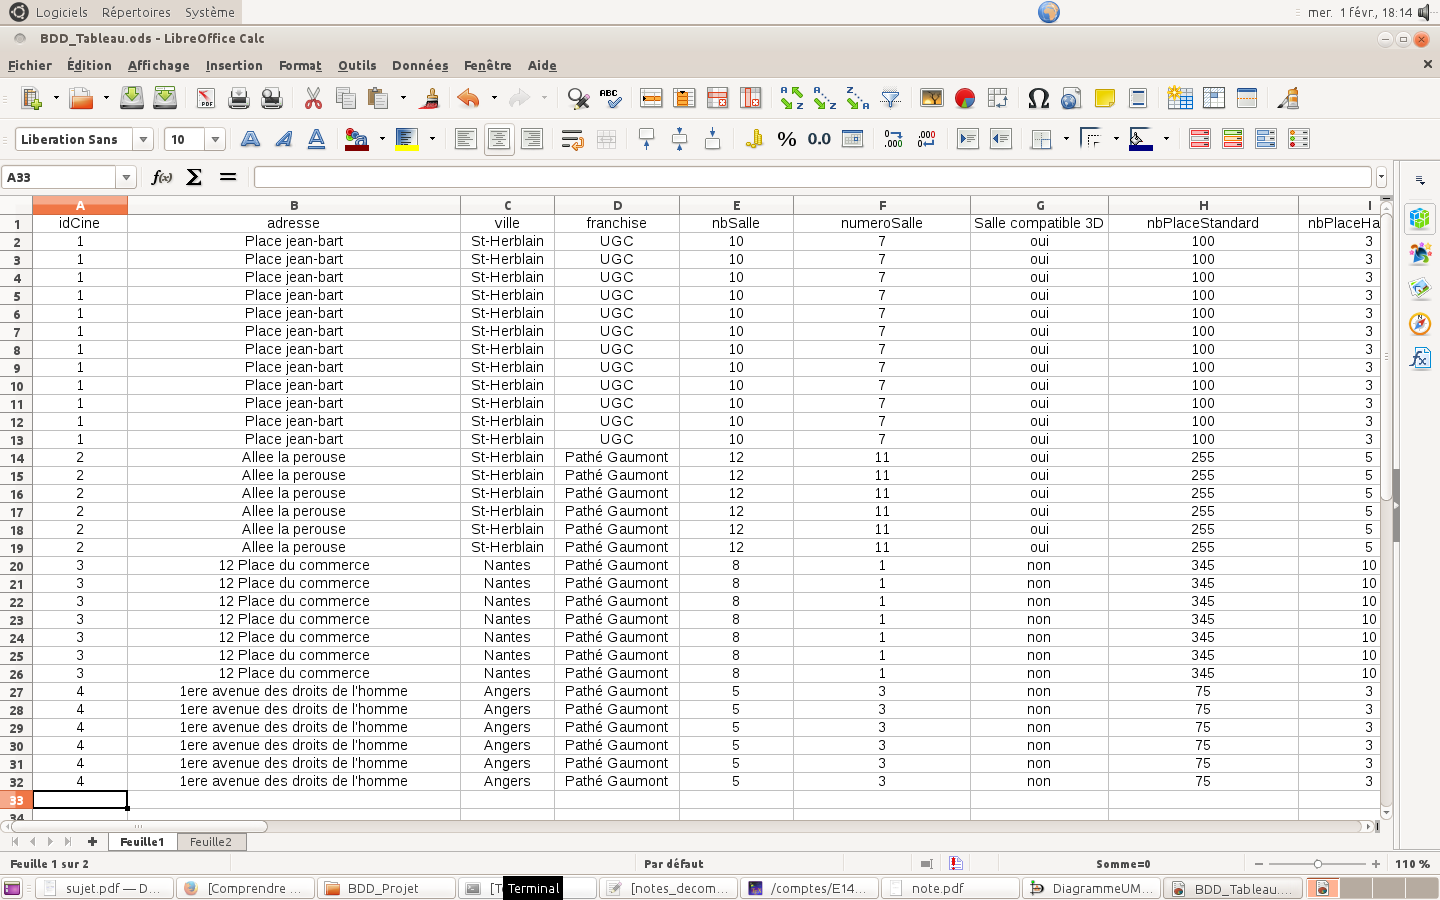
\includegraphics[height=9cm]{table_p1.png}}
			\caption{Première partie de notre table contenant tous les attributs et quelques tuples}
			\label{table_p1}	
		\end{figure}			
		
		\vspace{0.5cm}			

		\begin{figure}[!h]		
			\centerline{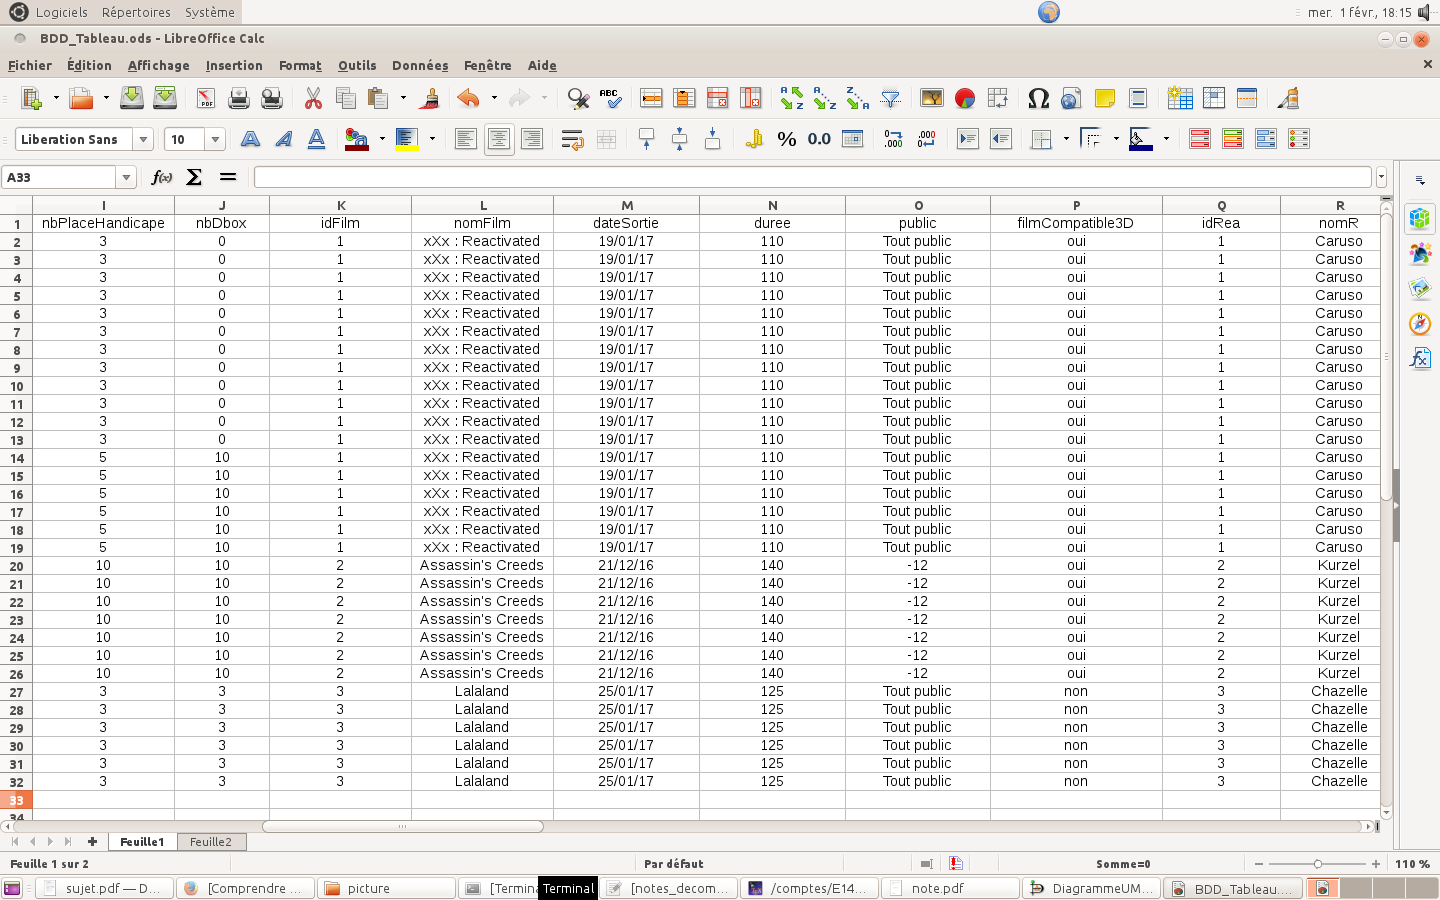
\includegraphics[height=9cm]{table_p2.png}}
			\caption{Deuxième partie de notre table contenant tous les attributs et quelques tuples}
			\label{table_p2}	
		\end{figure}			
		
		\vspace{0.5cm}

		\begin{figure}[!h]		
			\centerline{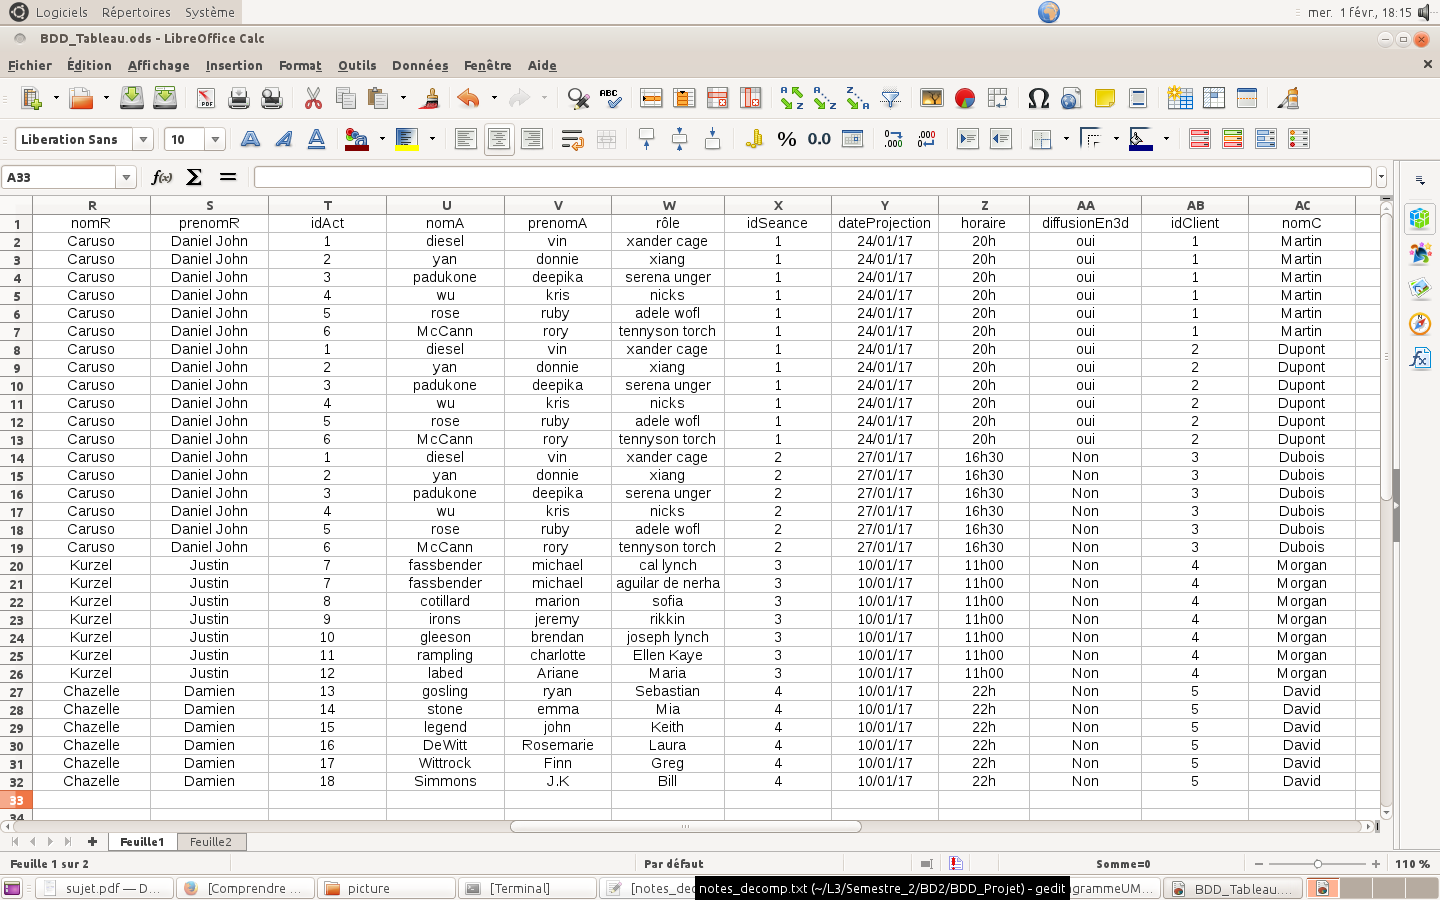
\includegraphics[height=9cm]{table_p3.png}}
			\caption{Troisième partie de notre table contenant tous les attributs et quelques tuples}
			\label{table_p3}	
		\end{figure}			
		
		\vspace{0.5cm}						

	\section{Dépendance fonctionnelle}
	
		\vspace{0.5cm}
	
		\noindent- (1) idCine $\rightarrow$ adresse, ville \\
		- (2) adresse, ville $\rightarrow$ franchise, nbsalle \\
		- (3) idCine $\rightarrow$ franchise, nbSalles \\
		- (4) idCine, numSalle $\rightarrow$ SallecompatibleEn3D, nbPlaceStandard, nbPlaceHandicape,nbDbox \\
 		- (5) idFilm $\rightarrow$ nomFilm, dateSortie \\
		- (6) nomFilm, dateSortie $\rightarrow$ public, idReal, duree, compatible3D \\
		- (7) idFilm, role $\rightarrow$  idAct \\
		- (8) idReal $\rightarrow$ nomR, prenomR \\
		- (9) idAct $\rightarrow$ nomA, prenomA \\
		- (10) idClient $\rightarrow$ nomC, prenomC \\
		- (11) idClient, numReservation $\rightarrow$ nbPlaceStandardRes, nbPlaceHandicapeRes, nbPlaceDBoxRes, idSeance \\
		- (12) idSeance, idCine $\rightarrow$ horaire, dateProjection, numSalle, idFilm, diffusionEn3D \\
		
	\section{Algo de Bernstein}
	
		\vspace{0.5cm}

		\noindent L'algo de Bernstein se fait en 4 parties : \\
			- Caclculer la CV(DF) et les clés. Si R est en 3FN, on s'arrête. \\
			- Partitionner CV(DF) e groupe DFi (1 <= i <= k) tels que toutes les df d'un même groupes aient la même partie gauche. \\
			- Construire un schéma <Ri(Ui), DFi> pour chaque groupe DFi, où Ui est l'ensemble des attribut apparaissant dans DFi. \\
			- Si aucun des schémas définis ne contient de clé X de R, rajouter un schéma <Rk+1(X), \{\}>. \\	

		\subsection{Caclcul de CV(DF)}

			\vspace{0.5cm}

			\noindent La couverture minimal se fait en trois parties : \\
				- Toutes les dépendances doivent être élémentaire ; les décomposer si nécessaire. \\
				- Eliminer les attributs superflus du coté gauche de la df. \\
				- Eliminer les dfs redondantes.
			
			\vspace{0.5cm}
				
			\subsubsection{pas 1}

				\vspace{0.5cm}

				\noindent- (1) idCine $\rightarrow$ ville \\
				- (1) idCine $\rightarrow$ adresse \\
				- (2) adresse, ville $\rightarrow$ franchise \\
				- (2) adresse, ville $\rightarrow$ nbsalle \\
				- (3) idCine $\rightarrow$ franchise \\
				- (3) idCine $\rightarrow$ nbSalles \\
				- (4) idCine, numSalle $\rightarrow$ SallecompatibleEn3D \\
		 		- (4) idCine, numSalle $\rightarrow$ nbPlaceStandard \\
		 		- (4) idCine, numSalle $\rightarrow$ nbPlaceHandicape \\
		 		- (4) idCine, numSalle $\rightarrow$ nbDbox \\
		 		- (5) idFilm $\rightarrow$ nomFilm \\
		 		- (5) idFilm $\rightarrow$ dateSortie \\				 		
				- (6) nomFilm, dateSortie $\rightarrow$ public \\
				- (6) nomFilm, dateSortie $\rightarrow$ idReal \\
				- (6) nomFilm, dateSortie $\rightarrow$ duree \\
				- (6) nomFilm, dateSortie $\rightarrow$ compatible3D \\
				- (7)idFilm, role $\rightarrow idAct$ \\
				- (8) idReal $\rightarrow$ nomR \\
				- (8) idReal $\rightarrow$ prenomR \\						
				- (9) idAct $\rightarrow$ nomA \\
				- (9) idAct $\rightarrow$ prenomA \\						
				- (10) idClient $\rightarrow$ nomC \\
				- (10) idClient $\rightarrow$ prenomC \\						
				- (11) idClient, numReservation $\rightarrow$ idSeance \\
				- (11) idClient, numReservation $\rightarrow$ nbPlaceStandardRes \\
				- (11) idClient, numReservation $\rightarrow$ nbPlaceHandicapeRes \\
				- (11) idClient, numReservation $\rightarrow$ nbPlaceDBoxRes \\
				- (12) idSeance, idCine $\rightarrow$ horaire \\
				- (12) idSeance, idCine $\rightarrow$ dateProjection \\
				- (12) idSeance, idCine $\rightarrow$ numSalle \\
				- (12) idSeance, idCine $\rightarrow$ idFilm \\
				- (12) idSeance  idCine $\rightarrow$ diffusionEn3D \\
		
				\vspace{0.5cm}
									
			\subsubsection{pas2}

				\vspace{0.5cm}
	
				\noindent - (2) adresse, ville $\rightarrow$ franchise, nbsalle \\
					\\
					\underline{adresse+} \\
					adresse \\
					\underline{ville+} \\
					ville \\
				$\rightarrow$ it's OK \\

				\noindent - (4) idCine, numSalle $\rightarrow$ SallecompatibleEn3D, nbPlaceStandard, nbPlaceHandicape,nbDbox \\
					\\
					\underline{idCine+} \\
					idCine / adresse / ville /franchise / nbSalle \\
					\underline{numSalle+} \\
					numSalle \\
				$\rightarrow$ it's OK \\
				
				\noindent - (6) nomFilm, dateSortie $\rightarrow$ public, idReal, duree, compatible3D \\																						\\
					\underline{nomFilm+} \\
					nomFilm \\
					\underline{dateSotie+} \\
					dateSortie \\
				$\rightarrow$ it's OK \\
			
				\noindent - (7) idFilm, role $\rightarrow$  idAct \\
					\\
					\underline{idFilm+} \\
					idFilm / nomFilm / dateSortie / public / idReal / duree / compatible3D / nomA / prenomA \\
					\underline{role+} \\
					role \\
				$\rightarrow$ it's OK \\
					
				\noindent - (11) idClient, numReservation $\rightarrow$ nbPlaceStandardRes, nbPlaceHandicapeRes, nbPlaceDBoxRes, idSeance \\
					\\
					\underline{idClient+} \\
					idClient / nomC / prenomC \\
					\underline{numReservation+} \\
					numReservation \\	
				$\rightarrow$ it's OK \\					
				
				\noindent - (12) idSeance, idCine $\rightarrow$ horaire, dateProjection, numSalle, idFilm, diffusionEn3D \\												
					\\
					\underline{idSeance+}
					idSeance \\
					\underline{idCine+}
					adresse / ville / franchise / nbSalle \\
				$\rightarrow$ it's OK \\

				\vspace{0.5cm}

			\subsubsection{pas3}		
	
				\vspace{0.5cm}
	
				\noindent Eliminons tout d'abord les dfs qui sont préservées par transitivité : \\
	
					\noindent- (1) idCine $\rightarrow$ adresse, ville \\
					- (2) adresse, ville $\rightarrow$ franchise, nbsalle \\
					- (3) idCine $\rightarrow$ franchise, nbSalles \\
					
					Si l'on prend les dfs 1, 2 et 3, on remarque que l'on peut supprimer la 3 car on peut retrouver celle-ci par transitivité. Reprenons donc nos dfs restantes : \\
					
				\noindent- (1) idCine $\rightarrow$ adresse, ville \\
				- (2) adresse, ville $\rightarrow$ franchise, nbsalle \\
				- (3) idCine, numSalle $\rightarrow$ SallecompatibleEn3D, nbPlaceStandard, nbPlaceHandicape,nbDbox \\
		 		- (4) idFilm $\rightarrow$ nomFilm, dateSortie \\
				- (5) nomFilm, dateSortie $\rightarrow$ public, idReal, duree, compatible3D \\
				- (6) idFilm, role $\rightarrow$  idAct \\
				- (7) idReal $\rightarrow$ nomR, prenomR \\
				- (8) idAct $\rightarrow$ nomA, prenomA \\
				- (9) idClient $\rightarrow$ nomC, prenomC \\
				- (10) idClient, numReservation $\rightarrow$ nbPlaceStandardRes, nbPlaceHandicapeRes, nbPlaceDBoxRes, idSeance \\
				- (11) idSeance, idCine $\rightarrow$ horaire, dateProjection, numSalle, idFilm, diffusionEn3D \\
				
				\noindent A présent, analysons chaque dfs une part une : \\
				
				\noindent - (1) idCine $\rightarrow$ adresse, ville \\
					\\
					\underline{idCine+} \\
					idCine\\									
				$\rightarrow$ it's OK \\		
					
				\noindent - (2) adresse, ville $\rightarrow$ franchise, nbsalle \\
					\\
					\underline{adresse+} \\
					adresse\\
					\underline{ville+} \\
					ville \\									
				$\rightarrow$ it's OK \\
				
				\noindent - (3) idCine, numSalle $\rightarrow$ SallecompatibleEn3D, nbPlaceStandard, nbPlaceHandicape,nbDbox \\
					\\
					\underline{idCine+} \\
					idCIne / adresse / ville / franchise / nbSalle\\
					\underline{numSalle+} \\
					numSalle \\								
				$\rightarrow$ it's OK \\													

				\noindent - (4) idFilm $\rightarrow$ nomFilm, dateSortie \\
					\\
					\underline{idFilm+} \\
					idFilm\\								
				$\rightarrow$ it's OK \\	
				
				\noindent - (5) nomFilm, dateSortie $\rightarrow$ public, idReal, duree, compatible3D \\
					\\
					\underline{nomFilm+} \\
					nomFilm \\
					\underline{dateSortie+} \\
					dateSortie \\									
				$\rightarrow$ it's OK \\	
				
				\noindent - (6) idFilm, role $\rightarrow$  idAct  \\
					\\
					\underline{idFilm+} \\
					idFilm / nomFilm / dateSortie / public / idReal / duree / compatible3D / nomR / prenomR \\
					\underline{role+} \\
					role \\									
				$\rightarrow$ it's OK \\																				
	
				\noindent - (7) idReal $\rightarrow$ nomP, prenomP \\
					\\
					\underline{idReal+} \\
					idReal \\								
				$\rightarrow$ it's OK \\	
				
				\noindent - (8) idAct $\rightarrow$ nomP, prenomP \\
					\\
					\underline{idAct+} \\
					idAct \\									
				$\rightarrow$ it's OK \\	

				\noindent - (9) idClient $\rightarrow$ nomC, prenomC \\
					\\
					\underline{idClient+} \\
					idClient \\									
				$\rightarrow$ it's OK \\		

				\noindent - (10) idClient, numReservation $\rightarrow$ nbPlaceStandardRes, nbPlaceHandicapeRes, nbPlaceDBoxRes, idSeance \\
					\\
					\underline{idClient+} \\
					idClient \ nomC \ prenomC \\
					\underline{numReservation+}
					numReservation \\									
				$\rightarrow$ it's OK \\		

				\noindent - (11) idSeance, idCine $\rightarrow$ horaire, dateProjection, numSalle, idFilm, diffusionEn3D \\
					\\
					\underline{idSeance+} \\
					idSeance \\
					\underline{idCine+}\\
					idCine \\ adresse \ ville \\ franchise \ nbSalle \\							
				$\rightarrow$ it's OK \\							
				\\		
				\noindent Ainsi, hormis la suppression de dfs transitives, nos dfs ne changes pas. \\																
				\\
				On constate que l'on est bien en 1FN, ainsi qu'en 2FN. Cependant nous ne sommes pas en 3eme forme normal. En effet, avec les dfs ci-dessus, nous obtenons la clé suivante : \{idCine, idClient, numReservation, role\}. \\
				Hors avec cette clé, nous avons des attributs non clés, qui déterminent d'autres attributs non clés. Par exemple, adresse et ville sont deux attributs non clé qui détermine franchise et nbSalle qui sont eux aussi non clés. \\
				
				\vspace{0.5cm}
													
			\subsection{Partitionnement de la CV et construction des schémas} 	
			
				\vspace{0.5cm}
			
				\noindent R1 = \{idCine, adresse, ville\} \\  DF1 = \{idCine $\rightarrow$ adresse, ville\} \\
				\\
				R2 = \{idCine, franchise, nbSalle\} \\ DF2 = \{adresse, ville $\rightarrow$ franchise, nbSalle\} \\
				\\
				R3 = \{idCine, numSalle, salleCompatibleEn3D, nbPlaceStanard, nbPlaceHandicapes, nbDbox\} \\ DF3 = \{idCine, numSalle, $\rightarrow$ salleCompatibleEn3D, nbPlaceStanard, nbPlaceHandicapes, nbDbox\} \\
				\\
				R4 = \{idFilm, nomFilm, dateSortie\} \\ DF4 = \{idFilm $\rightarrow$ nomFilm, dateSortie\} \\
				\\
				R5 = \{idFilm\} \\ DF5 = \{nomFilm, dateSortie $\rightarrow$ public, idReal, duree, compatible3D\} \\	
				\\							
				R6 = \{idFilm, role, idAct\} \\ DF6 = \{idFilm, role $\rightarrow$  idAct\} \\
				\\
				R7 = \{idReal, nomR, prenomR\} \\ DF7 = \{idReal $\rightarrow$ nomR, prenomR\} \\
				\\
				R8 = \{idAct, nomA, prenomA\} \\ DF8 = \{idAct $\rightarrow$ nomA, prenomA\} \\
				\\
				R9 = \{idClient, nomC, prenomC\} \\ DF9 = \{idClient $\rightarrow$ nomC, prenomC\} \\ 
				\\
				R10 = \{idClient, numReservation, nbPlaceStandardRes, nbPlaceHandicapesRes, nbPlaceDBoxRes, idSeance\} \\ DF10 = \{idClient, numReservation $\rightarrow$  nbPlaceStandardRes, nbPlaceHandicapesRes, nbPlaceDBoxRes, idSeance\} \\
				\\
				R11 = \{idSeance, idCine, horaire, dateProjection, numSalle, idFilm, diffusionEn3D\} \\ DF11 = \{idSeance, idCine $\rightarrow$ horaire, dateProjection, numSalle, idFilm, diffusionEn3D\} \\
				\\
				
				\vspace{0.5cm}
								
			\subsection{Ajout d'un schéma} 	

				\vspace{0.5cm}
											
				R12 = \{idCine, idClient, numReservation, role\} \\ DF12 = \{\} \\

				\vspace{0.5cm}

			\section{Algo de décomposition}

				\vspace{0.5cm}
	
\end{document}